\section{Data Structure}
The document is stored on disk in the form of a tree.  The root of the tree represents the document as a whole, and the document�s inode holds a pointer to this location on disk.  This location on disk, in turn, knows how many paragraphs the document contains, and contains pointers to each of the document�s paragraphs.  At the next level in the tree, each paragraph contains pointers to each sentence.  Finally, each sentence in the tree actually contains the data of individual sentences.  The concept of the tree is just a way of representing the data of a document.  By choosing to represent data in this manner, tasks such as merging and commiting code can be done in a very efficient manner.  Consider the following document. \\[18px]
\textit{The dog runs. The dog is fast.}\\[12px]
\textit{The cat naps.}\\[18px]
The previous document can be seen in Figure 1, in the form of the data structure that represents the document.

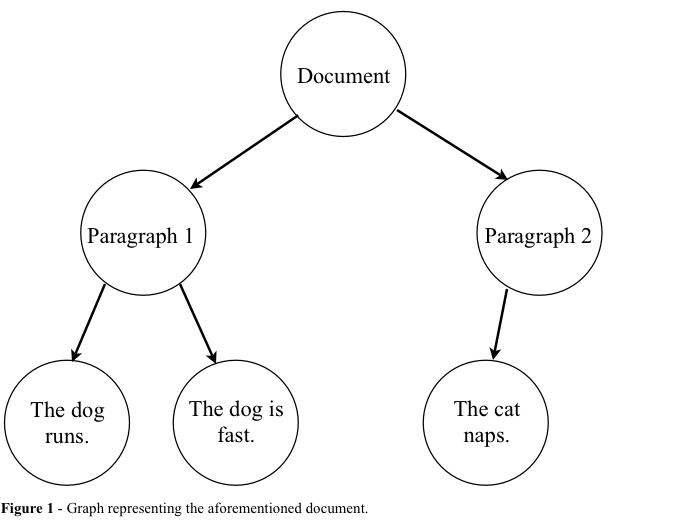
\includegraphics[scale=0.70]{graph1.png}